% This template was designed by Ruben De Smet. Visit his website at https://gitlab.com/rubdos/texlive-vub

\documentclass{beamer}

\usepackage{textpos}
\usepackage{selinput}
\usepackage{fontspec}
\usepackage{tikz}
\usepackage{graphicx}
\usepackage{minted}
\usepackage{svg}

\usefonttheme{professionalfonts} % using non standard fonts for beamer
\usefonttheme{serif}
\usepackage[justification=centering]{caption}

\newcommand*{\grabto}[2]{\IfFileExists{#2}{}{\immediate\write18{curl \detokenize{#1 -o #2}}}}


\tikzset{
    vertex/.style = {
        circle,
        fill            = black,
        outer sep = 3pt,
        inner sep = 2pt,
    }
}


% preloaded images
\grabto{https://upload.wikimedia.org/wikipedia/en/3/36/OTtp1.jpg}{OT-Operations-Order.jpg}
\grabto{https://upload.wikimedia.org/wikipedia/en/6/64/OTtp2.jpg}{OT-Transformation-Matrix.jpg}
%\usetheme{vub} % This will automatically load all fonts (Roboto and TeX Gyre Adventor
               % for titles), and the VUB colors. Also includes the triangle.
%\usetheme[coloredtitles]{vub}
%\usetheme[showsection]{vub}
\usetheme{Boadilla}
\makeatother
\setbeamertemplate{footline}
{
  \leavevmode%
  \hbox{%
  \begin{beamercolorbox}[wd=.5\paperwidth,ht=2.25ex,dp=1ex,center]{author in head/foot}%
    \usebeamerfont{author in head/foot}\insertshortauthor
  \end{beamercolorbox}%
  \begin{beamercolorbox}[wd=.6\paperwidth,ht=2.25ex,dp=1ex,center]{title in head/foot}%
    \usebeamerfont{title in head/foot}\insertshorttitle\hspace*{3em}
    \insertframenumber{} / \inserttotalframenumber\hspace*{1ex}
  \end{beamercolorbox}}%
  \vskip0pt%
}

\makeatletter


\setbeamertemplate{blocks}[rounded][shadow=false]
\addtobeamertemplate{block begin}{\pgfsetfillopacity{0.9}}{\pgfsetfillopacity{1}}

\setbeamertemplate{navigation symbols}{}
%\setmainfont{Helvetica Neue}
%\setmainfont{Palatino}
%\setbeamercolor{normal text}{fg=red}

%\setbeamerfont{headline}{family=\fontfamily{hn}\selectfont}
%\setbeamerfont{title}{family=\fontfamily{hvneue}\selectfont}
%\setbeamerfont{frametitle}{family=\fontfamily{hvneue}\selectfont}
%\setbeamerfont * {framesubtitle}{family=\fontfamily{hvneue}\selectfont}
\setbeamerfont{framesubtitle}{family=\fontspec{Helvetica Neue},size={\fontsize{7}{7}}}
\setbeamerfont{navigation symbols}{family=\fontspec{Helvetica Neue}}
\setbeamerfont{title in head/foot}{family=\fontspec{Helvetica Neue}}
\setbeamerfont{author in head/foot}{family=\fontspec{Helvetica Neue}}
\setbeamerfont{page number in head/foot}{family=\fontspec{Helvetica Neue}}

\setbeamercolor{page number in head/foot}{fg=white, bg=black}
\setbeamercolor{title}{fg=black}
\setbeamercolor{frametitle}{fg=black}
\setbeamercolor{navigation symbols}{fg=black, bg=black}
\setbeamercolor{structure}{fg=black}

\setmonofont{Monaco}

%%%%%%%%%%%%%%%%%%%%%%%%%%%%%%%%%%%%%%%%%
%%% CODE SNIPPETS                     %%%
%%%%%%%%%%%%%%%%%%%%%%%%%%%%%%%%%%%%%%%%%

\begin{VerbatimOut}{gcounter.js}
class GCounter {
  constructor(n) { this.n = n; }
  
  increment() { return new GCounter(this.n + 1); }
  
  query() { return this.n; }
  
  merge(counter) { 
    return new GCounter(
      Math.max(counter.query(), this.n));
  }
}
\end{VerbatimOut}


\begin{VerbatimOut}{pncounter.js}
class PNCounter {
  constructor(p, n) { this.n = n; this.p = p}
  
  increment() { return new PNCounter(
    this.p.increment(), this.n); }
    
  decrement() { return new PNCounter(
    this.p, this.n.increment()); }
    
  query() { return this.p.query() - this.n.query(); }
  
  merge(pncounter) {
    return new PNCounter(this.p.merge(pncounter.p),
                         this.n.merge(pncounter.n));
  }
}
\end{VerbatimOut}
%%%%%%%%%%%%%%%%%%%%%%%%%%%%%%%%%%%%%%%%%
%%%%  END OF CODE SNIPPETS            %%%
%%%%%%%%%%%%%%%%%%%%%%%%%%%%%%%%%%%%%%%%%


\title{Groupware Systems for fun and profit}
\subtitle{CRDT, OT, Quorum-commit etc.} % Can be omitted
\author{Max Klymyshyn}
\date{\today}



\begin{document}

\begin{frame}
\titlepage
\end{frame}



\begin{frame}{Groupware or Collaborative System}
\framesubtitle{synchronization in asynchronous environments}


\begin{block}{}
Real-time groupware systems are multi-user systems
where the actions of one user 
\textbf{must quickly be propagated to the other users}.
\end{block}

\vspace{0.5cm}
Examples of Groupware Systems:


\begin{itemize}
\item Any kind of chats with clients on \textbf{multiple devices}
\item Real-time group editing functionality (google docs etc.)
\item Real-time games
\item Conferences software
\item Notes, contacts, reminders, calendars
\item Shopping carts, group ordering
\end{itemize}

\end{frame}


\begin{frame}{Synchronization in asynchronous environment}
\framesubtitle{and different types of distributed replication approaches}

Here is list of basic problems within asynchronous setting:
\begin{itemize}
\item \textbf{conflicts} \small{\textit{when participants performing group activities}}
\item \textbf{unreliable networks} \small{\textit{primarily mobile clients with blinking connection}}
\item \textbf{offline activities} \small{\textit{allowing users to perform operations offline like editing text}}
\end{itemize}
\end{frame}

\begin{frame}{Replication and Consistency}
\framesubtitle{and different types of distributed replication approaches}
Basically there's only two hight-level approaches for replications: \textbf{Pessimistic} and \textbf{Optimistic} replications.
\vspace{0.5cm}
\begin{block}{Pessimistic Replication}
Or single-copy serializability: The idea is to prohibit access to a replica unless it is provably up to date. Techniques: two-phase commit, quorum-consensus, same-order delivery.
\end{block}
\vspace{0.5cm}
\begin{block}{Optimistic Replication or Eventual Consistency}
Updates sent asynchronously to other replicas;
every replica eventually applies all updates, possibly in different orders
\end{block}

\end{frame}


\begin{frame}{Naive approaches}
\framesubtitle{to organize synchronization within groupware systems}

\begin{itemize}
  \item Locking
  \item Transactions
  \item Single Active Participant
  \item Dependency Detection
  \item Reversible Execution
\end{itemize}

\end{frame}

\begin{frame}{Consistency Models}

\begin{itemize}
 	\item \textbf{Strong Consistency} – after the update completes, any subsequent access will return the updated value
	\item \textbf{Weak Consistency} – the system does not guarantee that subsequent accesses will return the updated value
	\item \textbf{Eventual Consistency} – eventually all accesses will return the last updated value.
	\item \textbf{Strong Eventual Consistency} – special case of EC which adds the safety guarantee that any two nodes that have received the same (unordered) set of updates will be in the same state
\end{itemize}

\end{frame}

\begin{frame}{Operation Transformation (OT) System Model}
\framesubtitle{and definitions}

\begin{block}{OT}
is a technology for supporting a range of collaboration functionalities in advanced collaborative software systems.	
\end{block}
\vspace{0.5cm}
\begin{itemize}
	
  \item Definitions
  \begin{itemize}
    \item Processes or sites are participants of the collaborative system
    \item Commands or operations are operations provided by system \textit{(for example insert text, delete text etc.)}
    \item Required properties and Transformations Matrices
  \end{itemize}     
\end{itemize}
\end{frame}

\begin{frame}{Transformation Property}

Operations must bee commutative:
\[op_1 \odot op_2 = op_2 \odot op_1\]

\begin{figure}
	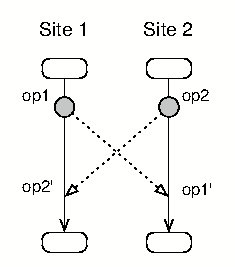
\includegraphics[scale=0.5]{OT-Operations-Order.jpg}
	\caption{order of operations for different sites}
\end{figure}

\end{frame}


\begin{frame}{Transformation Matrix}
\framesubtitle{formal definition}

\[o_{j}^{'} = T(o_j, o_i, p_j, p_i)\]
\[o_{i}^{'} = T(o_i, o_j, p_i, p_j)\]
\center{then \textbf{T} is such that following is satisfied:}

\[o_{j}^{'} \odot o_{i}^{'} = o_{i}^{'} \odot o_{j}^{'}\]


\end{frame}


\begin{frame}{Transformation Function picture}

\begin{figure}
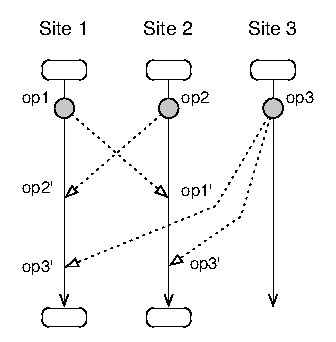
\includegraphics[scale=0.5]{OT-Transformation-Matrix.jpg}
\caption{Transformation Function}
\end{figure}

\end{frame}



\begin{frame}{OT Summary: Intention-violation}

\begin{itemize}
	\item Famous algos: GROVE, dOPT, Jupiter, adOPTed, REDUCE, GOT, GOTO
	\item Proving correctness of transformation functions is a complex task
	\item Impossible to establish proofs without computer within reasonable time for complex TF
	\item Following Oster et al. "Proving correctness of transformation functions in collaborative editing systems" paper only OT implementation of Tombstone Transformation Functions is correct
\end{itemize}
\end{frame}


\begin{frame}{Who is using OT?}

\begin{itemize}
	\item Google Docs
	\item ex-Google Wave
	\item A lot of other experiments
\end{itemize}
\end{frame}


\begin{frame}{OT Ressel et al. model}

\begin{columns}[c]
  \begin{column}{0.1\textwidth}    	
  \end{column}

  \begin{column}{0.4\textwidth}  
    \begin{figure}
      \centering    
	  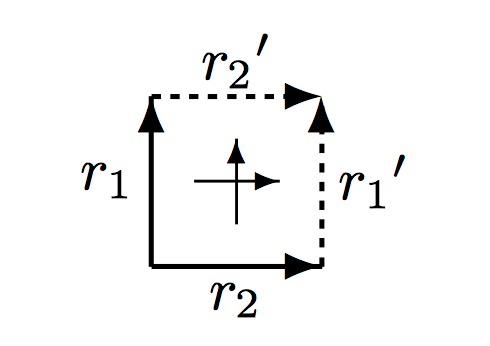
\includegraphics[scale=0.3]{OT-MatthiasRessel-2.png}    
      \caption{L-Transformation: $r_1 \odot r_2^{'} \equiv r_2 \odot r_1^{'}$}
    \end{figure}
  \end{column}

  \begin{column}{0.5\textwidth}
    \begin{center}
      \begin{figure}
        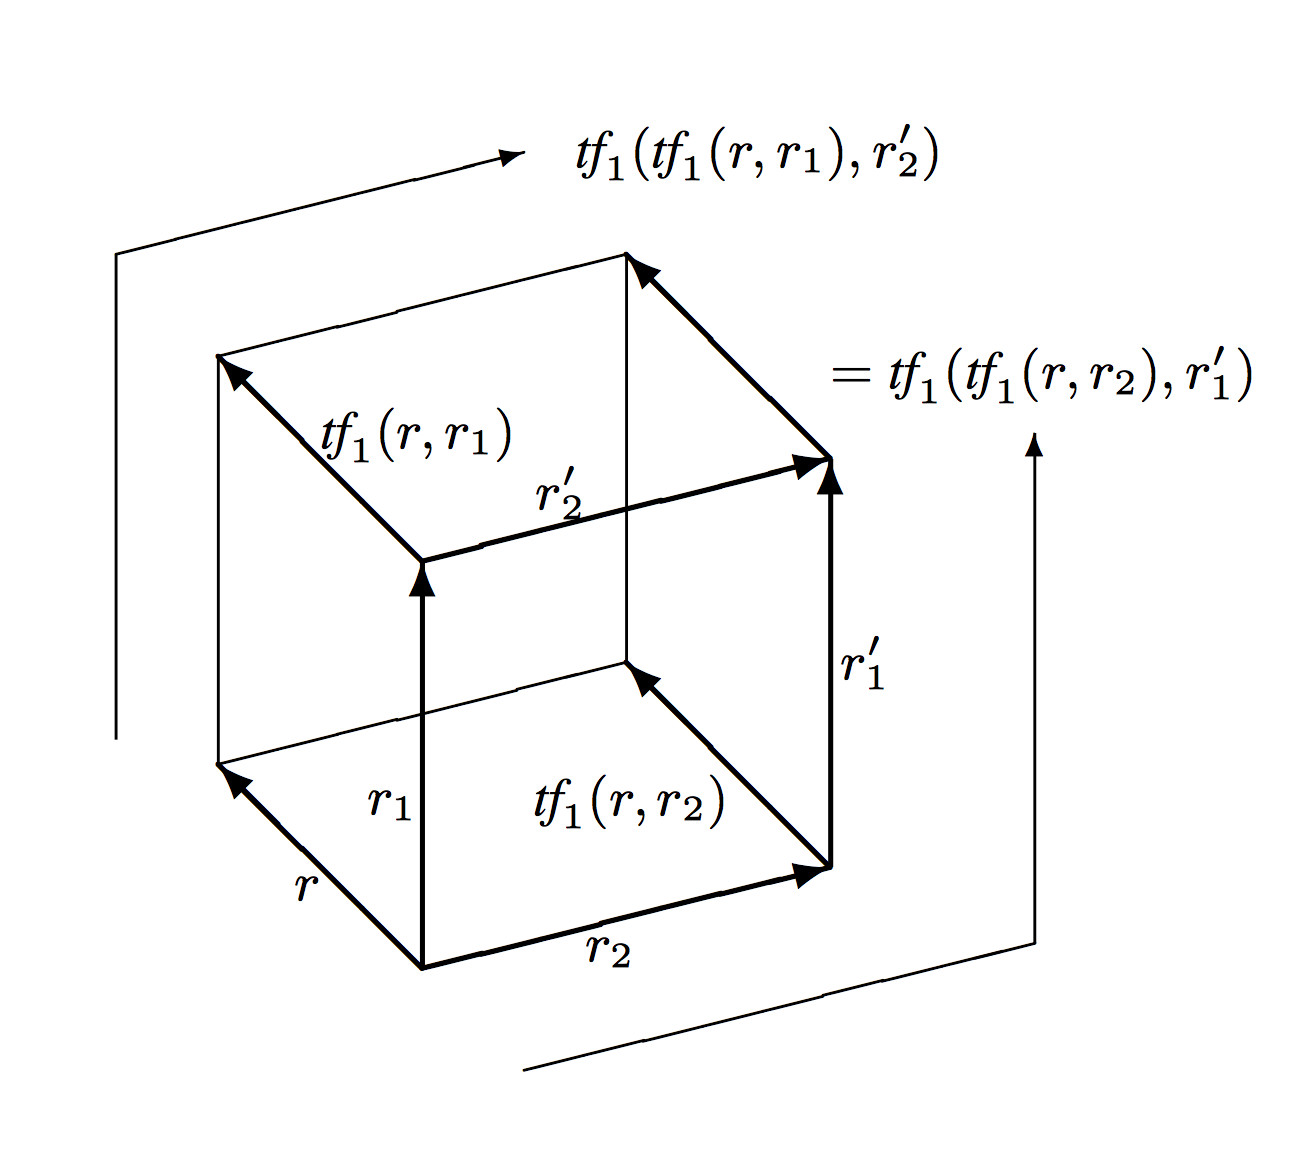
\includegraphics[scale=0.25]{OT-MatthiasRessel-1.png}
      \end{figure}
    \end{center}
  \end{column}
\end{columns}	

\end{frame}



\begin{frame}{Conflict-free replicated data types (CRDT)}
\begin{block}{CRDT is}
data type for the system of processes interconnected by an asynchronous network
where replicas can be updated independently and concurrently without coordination
between the replicas.
\end{block}
\vspace{0.5cm}
This kind of replication is very handy for client-side developers because:
\begin{itemize}
	\item Does not require active back-end system participation
	\item Quality leap in UX for users with weak or blinking network connections
	\item Better experience for SPAs with long single-load sessions like SoundCloud or GMail
	\item Offline work
\end{itemize}
\end{frame}


\begin{frame}{CRDTs: CvRDT, CmRDT}
\framesubtitle{state-based and op-based replication}

\begin{columns}[c]
  \begin{column}{0.4\textwidth}  
    \begin{figure}
      \centering    
	  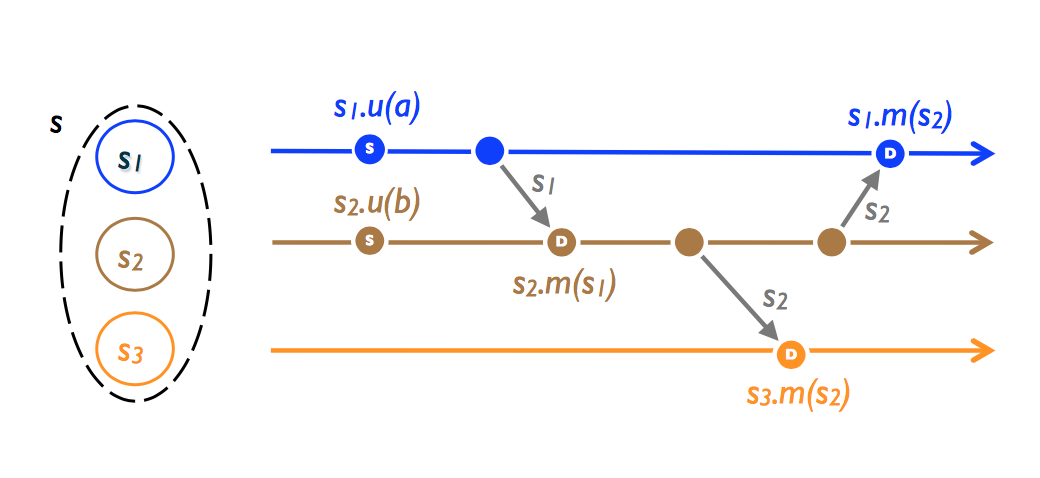
\includegraphics[scale=0.3]{CRDT-StateBased.png}    
      \caption{\textbf{State-based} Convergent Replicated Data Type or CvRDT}
    \end{figure}
  \end{column}

  \begin{column}{0.4\textwidth}
    \begin{center}
      \begin{figure}
        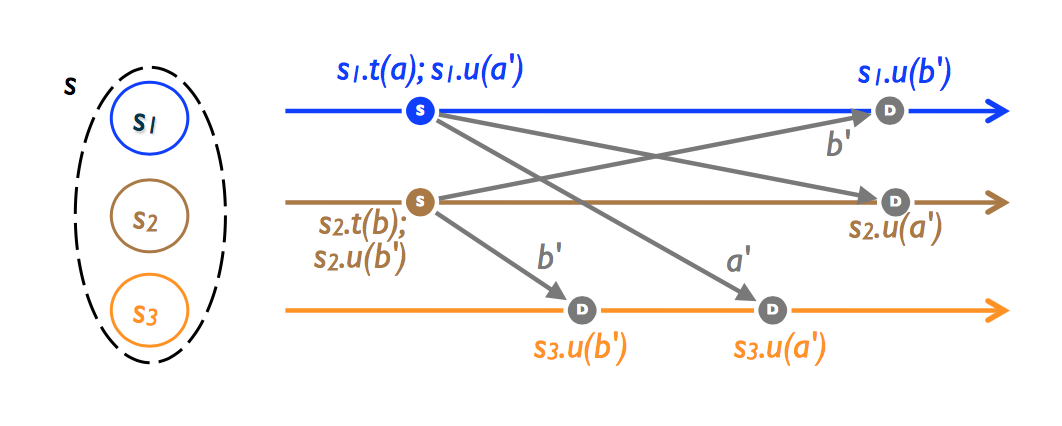
\includegraphics[scale=0.3]{CRDT-OP-Based.png}
        \caption{\textbf{Op-based} Commutative Replicated Data Type or CmRDT}
      \end{figure}
    \end{center}
  \end{column}
\end{columns}	


\end{frame}


\begin{frame}{CvRDT and CmRDT Properties}
\framesubtitle{Required properties}

$C(x_i)$ – Causal history of a replica $i$, 

\begin{itemize}
	\item \textbf{convergence} – $\forall i,j : C(x_i) = C(x_j)$
	\item \textbf{associativity} – nodes must come to the exactly same state regardless of the order they receive information: $a \odot b = b \odot a$, 
	\item \textbf{idempotency} – $a \odot a = a$
	\item least upper bound or LUB – $\sqcup_v$ which maintains
\end{itemize}

\begin{figure}[!ht]
	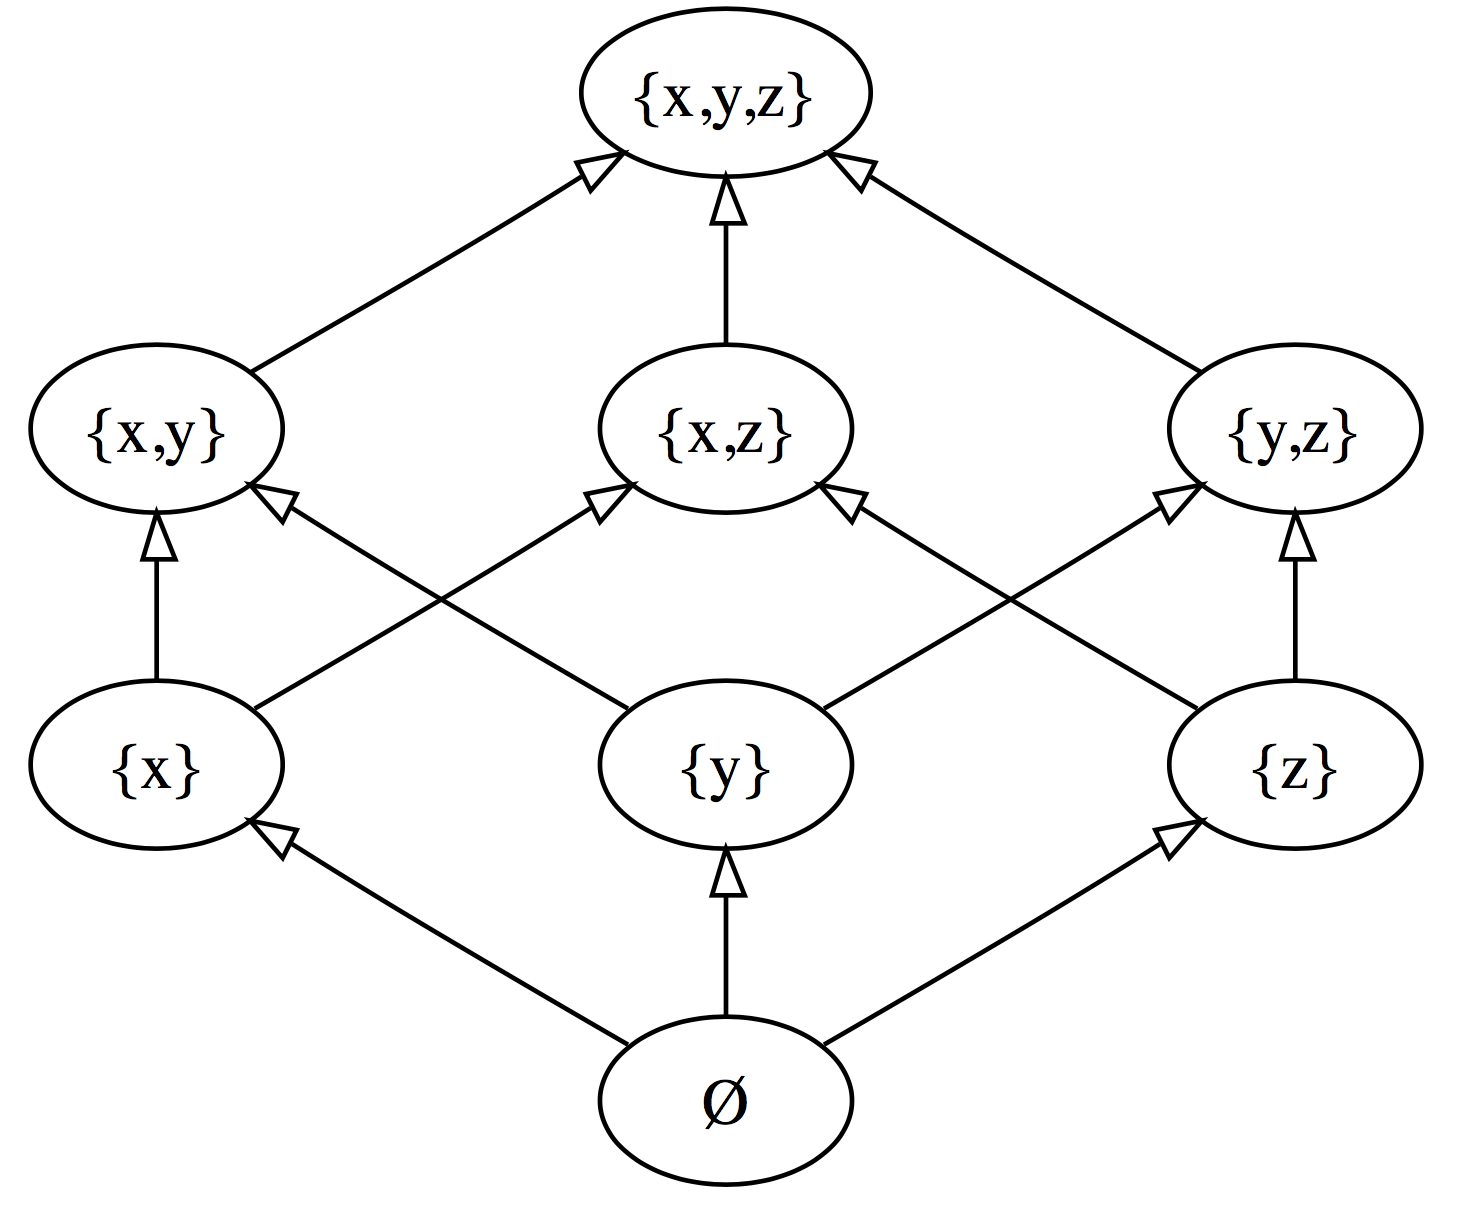
\includegraphics[scale=0.15]{LUB.png}    
	\caption{Least Upper Bound}
\end{figure}

\end{frame}


\begin{frame}{CRDT: GCounter}
\framesubtitle{Increment only counter}

\inputminted[
  firstline=1,
  framesep=0.5cm,
  frame=leftline,
  baselinestretch=1.1,
  fontsize=\scriptsize,
  rulecolor=\color{white}  
  linenos=true]{javascript}{gcounter.js}

\end{frame}

\begin{frame}{CRDT: PNCounter}
\framesubtitle{Increment and decrement counter}

\inputminted[
  firstline=1,
  framesep=0.5cm,
  frame=leftline,
  baselinestretch=1.1,
  fontsize=\scriptsize,
  rulecolor=\color{white}
  linenos=true]{javascript}{pncounter.js}
  
\end{frame}


\begin{frame}{Existing Tools}

\begin{itemize}
  \item ShareDB (and fall of Google Wave)
  \item Swarm (and forever-in-pre-alpha tool)
  \item OT.js (Operational Transformation for JS)
  \item CRDT – github.com/dominictarr/crdt
  \item replikativ.io – p2p distributed system framework
  \item other CRDT implementations
\end{itemize}

\end{frame}


\begin{frame}{Operation-based OR-Set}
\framesubtitle{Example of CmRDT data type (couple slides)}
\textit{Example add/remove set implementation in JS}
\end{frame}


\begin{frame}{Who is using CRDTs?}
\begin{itemize}
	\item \href{https://dzone.com/articles/facebook-announces-apollo-qcon}{Facebook}
	\item \href{https://speakerdeck.com/ajantis/practical-demystification-of-crdts}{TomTom}
	\item \href{http://highscalability.com/blog/2014/10/13/how-league-of-legends-scaled-chat-to-70-million-players-it-t.html}{League of Legends}
	\item \href{https://developers.soundcloud.com/blog/roshi-a-crdt-system-for-timestamped-events}{SoundCloud}
	\item \href{http://www.erlang-factory.com/static/upload/media/1434558446558020erlanguserconference2015bet365michaelowen.pdf}{Bet265}
	\item \href{http://docs.basho.com/riak/kv/2.2.3/developing/data-types/}{RIAK Distributed Database}
\end{itemize}
\end{frame}


\begin{frame}{References}

\begin{thebibliography}{1}

\bibitem{1} 
Marc Shapiro, Nuno Pregui ̧ca, Carlos Baquero, Marek Zawirski. 
\textit{A comprehensive study of Convergent and Commutative Replicated Data Types.} [Research Report] RR-7506, 2011, pp.50. <inria-00555588>

\bibitem{2} 
Yasushi Saito, Marc Shapiro
\textit{Replication: Optimistic Approaches}, HP Laboratories Palo Alto HPL-2002-33

\bibitem{3} 
Mihai Let, Nuno Pregui, Marc Shapiro
\textit{CRDTs: Consistency without concurrency control∗},

\bibitem{4}
Giuseppe DeCandia, Deniz Hastorun, Madan Jampani, Gunavardhan Kakulapati, Avinash Lakshman, Alex Pilchin, Swaminathan Sivasubramanian, Peter Vosshall and Werner Vogels
\textit{Dynamo: Amazon’s Highly Available Key-value Store}, Amazon.com

\bibitem{5}
G ́erald Oster, Pascal Urso, Pascal Molli, Abdessamad Imine. 
\textif{Real time group editors without Operational transformation.}
 [Research Report] RR-5580, INRIA. 2005, pp.24.

\bibitem{6}
Gérald Oster, Pascal Urso†, Pascal Molli, Abdessamad Imine
\textif{Proving correctness of transformation functions in collaborative editing systems}
Thèmes COG et SYM — Systèmes cognitifs et Systèmes symboliques
Projets ECOO et CASSIS, Rapport de recherche n° 5795 — Décembre 2005

\bibitem{7}
Paulo S ́ergio Almeida, Ali Shoker, and Carlos Baquero
\textif{Efficient State-based CRDTs by Delta-Mutation}
HASLab/INESC TEC and Universidade do Minho, Portugal 2015

\end{thebibliography}	

\end{frame}

\begin{frame}
\center{Thanks}
\center{@maxmaxmaxmax}
\end{frame}


\end{document}


